\documentclass[conference]{IEEEtran}
\IEEEoverridecommandlockouts
% The preceding line is only needed to identify funding in the first footnote. If that is unneeded, please comment it out.
\usepackage{cite}
\usepackage{float}
\usepackage{amsmath,amssymb,amsfonts}
\usepackage{algorithmic}
\usepackage{graphicx}
\usepackage{textcomp}
\usepackage{xcolor}
\usepackage{comment}
\usepackage{longtable}  
\def\BibTeX{{\rm B\kern-.05em{\sc i\kern-.025em b}\kern-.08em
    T\kern-.1667em\lower.7ex\hbox{E}\kern-.125emX}}
\begin{document}

\title{Towards a Modular IoT System Architecture  for Rural Aqueducts Using Model Based Systems Engineering\\
\thanks{Project funded by: TEC-Costa Rica Proyecto VIE 1341030}
}

\author{
\IEEEauthorblockN{Anthony José Arguedas-Rodríguez}
\IEEEauthorblockA{
\textit{Tecnológico de Costa Rica}\\
Cartago, Costa Rica \\
https://orcid.org/0009-0002-1662-1656}
\and
\IEEEauthorblockN{María José Angulo-Campos}
\IEEEauthorblockA{
\textit{Tecnológico de Costa Rica}\\
Cartago, Costa Rica \\
https://orcid.org/0009-0005-5842-1101}
\and
\IEEEauthorblockN{Juan José Montero-Jiménez}
\IEEEauthorblockA{
\textit{Tecnológico de Costa Rica}\\
Cartago, Costa Rica \\
https://orcid.org/0000-0002-3215-3736}
\and
\IEEEauthorblockN{Juan José Rojas-Hernádez}
\IEEEauthorblockA{
\textit{Tecnológico de Costa Rica}\\
Cartago, Costa Rica \\
https://orcid.org/0000-0002-3261-5005}
}

\maketitle

\begin{abstract}
\begin{comment}
Rural aqueducts are a lifeline for the communities they serve. They are responsible for managing critical water resources yet their monitoring processes are slow and costly, making water loss a common problem. Internet of Things (IoT)-enabled systems stand as a viable solution for improving water management. However, the design complexity of such systems is beyond the capabilities of most rural aqueducts, where needs are empirically well-known but not formally translated into technical requirements and then into solution architectures.

In this research, a potential solution using Model-Based System Engineering as frameworkto the generic and modular architecture of an IoT system is proposed for rural aqueducts. T

we identify model-based systems engineering (MBSE), based on the ARCADIA method and tooled by the Capella software, as a framework suitable for guiding the entire architecture design process for rural aqueduct IoT solutions targeting water monitoring and loss control. We detail our systematic application of the method to derive requirements from informally defined customer needs, then fulfilled by a logical architecture. We demonstrate that the obtained architectures are particularly valuable for rural aqueduct application due to being modular and tailored to specific end-user needs and desires. We furthermore show that the architectures and their design process are implementable and explainable by undergraduate students, which, within a framework of technology transfer, we frame as the most fitting adopters of the presented MBSE methodology to develop solutions for generally underserved rural aqueducts. We elaborate on needs and desires definition, systematic design, and the involvement of academia for architecture realization, thus presenting an end-to-end solution for rural aqueducts aiming to solve problems with IoT.    
\end{comment}
Rural aqueducts play a vital role in sustaining the communities they serve by managing the essential water resource. A common challenge for rural aqueducts is related to water loss and rudimentary monitoring methods. Internet of Things (IoT) enabled systems offer a promising solution to improve water management, yet their design complexity and costs often exceed technical and financial capacities in rural aqueducts.  This study proposes a Model-Based Systems Engineering (MBSE) approach to develop a modular IoT architecture tailored to rural aqueducts. Using the ARCADIA methodology and the Capella modeling tool, the process translates informal user needs into structured requirements and logical system designs. The resulting architectures are modular, adaptable, and aligned with end-user conditions. The methodology is accessible enough to be implemented by undergraduate students, positioning academic institutions as effective intermediaries for technology transfer. By formalizing needs and systematically guiding architecture development, MBSE offers a structured pathway to create IoT solutions for water monitoring and loss prevention. This approach provides a scalable, explainable framework to support the modernization of rural aqueduct systems.
\end{abstract}

\begin{IEEEkeywords}
rural aqueducts, internet of things, model-based systems engineering, technology transfer, water management
\end{IEEEkeywords}

\section{Introduction}
Water is an indispensable natural resource for life on Earth, and access to safe drinking water is both a basic human need and a fundamental right \cite{un_resolution_2010}. Ensuring the availability and quality of water is essential for the well-being and development of any population. Yet, for many rural communities worldwide, this remains a critical challenge.

In these communities, the problem is often related not only to water scarcity but also to the lack of adequate infrastructure for collection, treatment, and distribution \cite{10.2166/washdev.2025.299} \cite{gaviria-montoya_risk_2020}. The responsibility for managing and maintaining this infrastructure frequently falls to locally administered rural aqueducts, which operate with limited resources, outdated technologies, and low operational efficiency. These limitations contribute to issues such as water loss and unreliable service.

The Internet of Things (IoT) offers a promising means to address these limitations. Through automated monitoring and anomaly detection, IoT technologies can significantly enhance operational efficiency in rural aqueducts \cite{6844741}. However, high costs and limited customization options make commercial IoT solutions largely inaccessible for these small-scale systems.

Developing low-cost, tailored IoT solutions represents a feasible alternative to support rural aqueducts. In this context, Systems Engineering may offer a structured approach to guide the development of these solutions, ensuring that technical, operational, and contextual factors are properly considered.

Academic institutions, particularly through student-led technology transfer initiatives, can play a key role by contributing technical expertise and promoting the use of systematic development methodologies. One of the main motivations of the current work are multiple independent student initiatives of IoT Systems for rural aqueducts \cite{Oviedo2024} \cite{Solorzano2021}. This enhances both the educational impact and the likelihood of producing reliable, scalable, and context-appropriate IoT systems.

To this end, this work proposes a generic system architecture for rural aqueducts developed using the ARCADIA method \cite{arcadia}, a Model-Based Systems Engineering (MBSE) methodology. This architecture is intended to serve as a foundation for the design of modular IoT systems that address the specific challenges faced by rural aqueducts. The remainder of this paper is organized as follows: Section II presents the context of IoT systems for rural aqueducts and provides an overview of the current state of the art. Section III is dedicated to the proposed modular IoT system architecture for rural aqueducts. This section is divided in four parts, the theory background on system architecture based on ARCADIA method, the requirements analysis derived from initial needs and desires for the IoT system, the modular architecture proposal using ARCADIA method, and the implementation on a real case study for the physical architecture. Section IV is dedicated to the analysis and discussion on the proposed architecture. Finally, Section V concludes the paper and outlines future research directions.   

%Globally, rural communities face a significant crisis in access to sufficient and safe drinking water. Surprisingly, even in regions with abundant sources of clean water, the lack of adequate infrastructure for its collection and distribution can severely hamper access.
%In this context, the responsibility for managing, maintaining and improving such infrastructure often falls to rural aqueducts. Unlike urban or integrated areas, these entities are locally managed and financed, operating with constrained infrastructure and budgets that reflect their limited scope.

%These inherent limitations of rural aqueducts make them prone to depend on obsolete technologies and operational processes. This translates into low operational efficiency and exacerbates water resource management issues, including water loss.
%This is where Internet of Things (IoT) systems emerge as a promising solution. By enabling the automation of monitoring and anomaly detection through intelligent components, IoT can drastically improve operational efficiency across many rural aqueduct tasks.

%However, the limited funding of most rural aqueducts represents a significant barrier to the adoption of IoT solutions. Purchasing commercial, off-the-shelf IoT solutions is the simplest option, but their prohibitive costs and the lack of offerings tailored to the scale and specific needs of rural aqueducts make them unaffordable. Given this reality, a promising alternative emerges: the development of IoT systems designed specifically for rural aqueducts using low-cost components. This approach prioritizes cost-effectiveness and avoids oversizing.
%Considering that most rural aqueducts lack personnel dedicated to the design and development of IoT systems, these activities could be undertaken by academic actors, especially university students, within a technology transfer network. This synergy leverages the technological knowledge of universities and the initiative of many students, particularly undergraduates, who seek to gain experience in high-impact projects. 

%Given the criticality of the operations of rural aqueducts, technology transfer projects can not be limited to designing and implementing IoT solutions, but they must also demonstrate their robustness and fit for purpose even if they do not have a contractual obligation to do so as it would be the case for commercial parties.
%One strategy to accomplish this, and the one that will be followed in this work, is to avoid redesigning systems from the ground up for each technology transfer project, and to build upon previously published architectures which have already been subject to peer review, and, potentially, to actual implementation.

%For these rural aqueduct IoT architectures to serve as building blocks for individual for robust and fit-for-purpose implementations, they must be generic and modular. In this case, generality refers to encompassing the breadth of needs and desires experimented by rural aqueducts worldwide, as expressed by the literature.
%Generality also entails a separation between the core needs and desires of rural aqueducts, which aretaken to be shared among them worldwide, and their enabling technologies, between which rural aqueducts might make choices based on criteria too specific to be discussed in the literature, or that might be dependent on the technological landscape at one particular point in time. On the other hand, modularity is the quality that enables needs and desires to be complementary yet independent of each other, so that any technology transfer project can work only with a subset of them selected to best utilize monetary and development resources and avoid oversizing.

%However, technology transfer projects between universities and rural aqueducts are often presented as single case studies, focusing mostly on providing a proof of concept of the applicability of novel technologies and components in the context of IoT for rural aqueducts.
%In these cases, the proposed solutions are intentionally very different from previous work and thus can not be part of a continuing effort towards increasingly more trustworthy systems, leaving the responsibility of demonstrating their robustness and fit for purpose on the stakeholders of each new publication.


\begin{comment}
For the ideation of such architectures, model-based systems engineering, especially as described by the ARCADIA method, emerges
as an authoritative theoretical framework.
Through the concept of operational need analysis, this methodology allows for the study of not only diverse and generic needs and
desires, but also for their analysis in context, separating the technologies 

This implies that, in order to replicate these systems, rural aqueducts need to develop a deep technical understanding to assess how well
specific IoT system designs meet their requirements, which are most often not expressed in terms of the
technologies implemented but in terms of the operational capabilities they provide.

Expanding on the above in can be understood that another requirement for genericity  

Furthermore,for techIoT solutions, it is crucial that the real needs and wants of rural aqueducts are explicitly defined and understood. Although these needs are known empirically, aqueducts often have difficulty formalizing them themselves. Because rural aqueducts operate under radically different conditions worldwide, the IoT systems they implement must be inherently generic and modular. Generality refers to the ability to be applicable to actors with diverse needs, desires, operational activities and organizational structures, while modularity is defined as a requirement that explains how needs and desires are integrated into the logical architecture, allowing for their addition or removal as needed.\\

This is where Model-Based Systems Engineering (MBSE), particularly the ARCADIA method, becomes fundamental.
MBSE facilitates a deep understanding of the real needs and desires of rural aqueducts, formalizing
them as organizational models.
T
By incorporating generality and modularity as intrinsic needs, the MBSE method integrates them into the resulting IoT systems. The systematic application of an MBSE methodology not only brings credibility to the work done by students, but also facilitates the continuity of these projects by future generations of students, and even the technology transfer methodology itself can be modeled using MBSE for further guidance.


The purpose of the this work is to present a generic and modular IoT architecture for rural aqueducts, derived via the ARCADIA model-based method.
The motivation is that future technology transfer projects could implement this generic architecture in specific
rural aqueducts and disclose its practical strengths and weaknesses, so that a incremental
and collaborative demonstration of its robustness and fulfillment of rural aqueduct needs
and desires can arise.
By the virtue of adopting the evidence-proven architecture, all such technology transfer
could make a reliability guarantee to the rural aqueducts they work with, without
sacrificing cost efficiency and suitability.

For this effort, the ARCADIA MBSE method is instrumental for formalizing stakeholder
needs and desires and the model language used to describe the architecture that
fulfills these requirements, and implementing a multi-viewpoint engineering approach that can cover the various
perspectives through which this system can be analyzed, namely: modularity, and suitability
for technology transfer projects between universities and rural aqueducts.
Furthermore, adhering to the ARCADIA method straightens the path for any future work regarding context-specific
implementations of this generic and modular architecture, since it prescribes the approach to instantiate
generic system behavior into a physical, deployable system through the concept of a physical architecture.
\end{comment}
\begin{comment}
    
\indent Therefore, this paper will develop a generic IoT system for rural aqueducts following the ARCADIA method. A deep understanding of needs and wants will be achieved using data mining techniques (BERTopic). Subsequently, system architectures and logics will be developed, explicitly addressing generality and modularity. The MBSE-based architecture will allow rural aqueducts to determine their applicability by comparing their needs and wants with those presented here. It will also provide a solid foundation for university students to act as development partners, translating the logical architecture into a physical architecture specific to each rural aqueduct, and demonstrating its suitability.

% ------------------- Texto viejo, ignorar
Worldwide, rural populations are the most affected by a lack of sufficient and potable water.
The roots of this problem are many, encompassing climate change, water source pollution,
water loss, and the inadequacy of water distribution systems.
Even in areas with clean and abundant water sources, a lack of collection and supply infrastructure
can severely impact access to water.

In many jurisdictions, the responsibility of implementing, maintaining and improving water infrastructure
belongs to rural aqueducts, in contrast to to the areas where extensions of urban supply systems or
urban-rural integrations exist.
Rural aqueducts are locally managed and financed entities that operate solely for the community
they are located in, with infrastructure and budgets that reflect their limited scope.

The constraints of rural aqueducts make them prone to using outdated technology and operational processes, with an associated low operational efficiency and an increased risk of water loss, among other water resource management issues.

IoT systems can improve operational efficiency for all tasks that must be carried out by
rural aqueducts, mainly by automating monitoring and anomaly detection activities using
smart components.
IoT systems provide fast response times even across large service areas, something
especially influential given the low headcount of many rural aqueducts.

However, the limited funding of most rural aqueducts hinder their access to IoT systems,
instead relying on outdated technology and manual operational activities.
Purchasing commercial and implementation-ready IoT solutions is the simplest solution,
but prohibitive costs and a lack of private offers tailored to the scale and needs of
rural aqueducts leave them out of reach in many instances.

Thus, a promising alternative is to develop purpose-built IoT systems for rural aqueducts
using low-cost components, avoiding over-dimensioning and prioritizing cost-effectiveness.
With most rural aqueducts not having dedicated staff for IoT system design and development,
these activities could be better carried out by academic actors, mainly university students,
within a network of technology transfer.
Such an approach benefits from harnessing the technological expertise of universities and
the initiative of many students, particularly at the undergraduate level, to gain
experience working on high-impact projects.

Technology transfer projects between universities and rural aqueducts, however,
are often presented as one-off implementations, and they focus mostly on explaining the functionality of
systems in terms of the specific technologies and components implemented rather than presenting generic and modular
architectures that could be implemented in various contexts.
Thus, for rural aqueducts to replicate these systems they need a deep technical understanding of them,
to determine 

Various stakeholders, such as university students,
could be framed as technological design and development partners, but
they struggle with formalizing their proposals and demonstrating
robustness.
Undergraduate students are suitable partners for formalizing requirements, designing architectures, and implementing products, all grounded in technology transfer.

In both cases, it is crucial that the true needs and desires of rural aqueducts be explicitly
defined and understood.
The needs and desires of rural aqueduct stakeholders are well-known empirically but they struggle to formalize them on their own.
Thus, rural aqueducts can be assured that their IoT solutions are fit for their purpose,
regardless of who builds them or their price point.

Rural aqueducts are present worldwide and operate under radically different conditions.
Thus, the IoT systems they implement must be generic and modular.


Define generality as being applicable to stakeholders with different needs, desires, operational activities, and organizational structures.

Define modularity as a requirement, such that we explain how needs and desires permeate into the logical architecture, and how these can be added and removed on demand.

What is model-based systems engineering.
What is the ARCADIA MBSE method.

MBSE helps to understand true rural aqueduct needs and desires.
Generality and modularity can be incorporated as needs and the MBSE method will imbue them
into the derived IoT systems.

\textit{Who} applies a systems engineering methodology is relevant as it influences existing technical expertise and the set of suitable solutions for the logical architecture stage. \cite{se-mse}

Systematically following an MBSE methodology provides credibility to the work done by students, and also facilitates the continuation of these projects by the following generations of students.

The technology transfer methodology itself can be modeled using MBSE, for deeper guidance for students. \cite{7302801}

Thus, this paper will develop a generic IoT system for rural aqueducts following the ARCADIA method.
A deep understanding of needs and desires will be achieved by using data mining techniques (BERTopic).
Then, system and logical architectures will be developed, addressing genericity and modularity.

The MBSE-based architecture will allow rural aqueducts to determine if the architecture applies to them by comparing their
needs and desires to the ones presented here.
University students will be able to work as development partners by translating the presented
logical architecture into a physical architecture for a specific rural aqueduct.
They will be able to demonstrate that their physical architecture meets aquduct needs.

\end{comment}
\section{IoT Systems for rural aqueducts context}

The implementation of IoT systems for rural aqueducts is not new. In the last decade, multiple research initiatives have been developed and published. To ensure novelty on the work that is presented in this research, a complete and impartial search on previous studies has been conducted. Two research questions were proposed as a starting point for the literature survey:

\begin{itemize}
        \item \textbf{RQ1:} Are there existing systems engineering-based (including ARCADIA MBSE) architectures for the design of IoT systems for rural aqueducts?
        \item \textbf{RQ2:} If they exist, are the architectures generic and modular?
\end{itemize} 

Based on the research questions, a search on Scopus indexed publications was conducted based on title, abstract and keywords. The search queries were the following: 
\begin{itemize}
    \item ``rural aqueduct" IoT architecture, ``water distribution system" IoT architecture rural, ``rural water supply" IoT architecture
    \item ``systems engineering" IoT architecture ``rural aqueduct", ``systems engineering" ``water distribution system" rural IoT, ARCADIA IoT architecture, ARCADIA ``rural aqueduct" IoT, ``model-based systems engineering" IoT rural water 
\end{itemize}

The inclusion criterion was that the results had to be related to IoT systems and some aspect of water distribution systems, rural or not. The results of the search showed that three out of the eight queries for RQ1 and RQ2 returned zero results, and for the remaining five queries, a total of 75 results were retrieved.
Out of these, only 21 met the inclusion criterion, and the most pertinent are presented below.

A systematic review by \cite{w14223621} provides a broad overview of IoT-based water monitoring and distribution systems, addressing applications, sensor technologies, and the role of artificial intelligence. However, no formal or generic architecture is proposed, though the need for such a framework is acknowledged. Similarly, \cite{Maroli2021Framework} presents a methodology for designing IoT-based rural water distribution systems, applied to a case study in India. Despite its claims of generality, the work lacks a formal, layered architecture and systematic derivation from stakeholder requirements.

Paper \cite{98953990} presents the IoTA4IWNet WDS architecture, which aims to provide a structure for water distribution systems with four distinct planes: edge, fog, cloud, and service. While its modularity and generality are suggested through broad technological coverage, no systems engineering approach is used, and no clear process is provided to adapt the architecture to specific stakeholder needs. In \cite{fi12070114}, another IoT architecture is presented named the REFlex Water architecture. The study introduces physical, middleware, and application layers, emphasizing flexibility through declarative process models. However, the work lacks systematic guidance for translating stakeholder needs into system design.
Similarly, \cite{10042624} proposes a layered IoT architecture with modules for monitoring, control, and data management. While modular in structure, the absence of a formal methodology or modeling language limits its adaptability. A more formal approach is seen in the BRAIN-IoT framework by \cite{tao-mbse}, which employs multiple formal modeling languages to structure system, software, and physical layers. Although grounded in systems engineering principles, the work does not follow ARCADIA, and the procedure for incorporating stakeholder needs is not detailed. Another example is found in \cite{10.13189/ujar.2022.100302}, which describes a IoT-based water management tools for rural communities in India, focusing on water level monitoring. Despite claiming generality, the architecture is specific to the technology used, with no formal mechanisms for adaptation beyond basic configuration.

None of the reviewed studies explicitly apply the ARCADIA MBSE method or systematically integrate generality and modularity as architectural requirements. While some works imply modularity or use formal modeling, they do not provide structured, traceable processes to connect stakeholder needs with system behavior, leaving this task to the reader. The current work addresses the identified gaps in these existing generic architectures.

%Most of the consulted studies shown that, the research efforts have been oriented at presenting designs only applicable in a particular context and under specific technological choices. 


%Whereas most of the literature at the crossroads between IoT and rural aqueducts is concernedwith presenting , the focus of this work is on generalizing rural aqueduct needs and desires,and eliciting a system architecture that can fulfill them in a modular manner via the ARCADIA MBSE method.

%To search for previous work on this front and assess the novelty of the present work, the following research questions wereposed:



%To tackle the research questions, a literature review was carried out via Scopus title-abstract-keywords searches.






%\subsection{Existing systems engineering-based frameworks for IoT systems for rural aqueducts}


%Paper \cite{w14223621} undertake a systematic literature review on IoT-based water monitoring systems (WMS) and water distribution systems (WDS), categorizing them in terms of applications, sensor and communication technologies, and AI- vs. non-AI-based systems. While this review does not aim to detail a particular implementation, less so a generic architecture, this work highlights the need for a generic framework that can guide data-processing and sensor equipment selection.

%In \cite{Maroli2021Framework}, the authors propose a general methodology intended to guide the design and implementation of IoT-based systems for rural water distribution, which they then apply to a specific case study village in India. Despite the authors' claims, this work does not present a formal, layered architecture in the typical systems engineering sense. Instead, it presents a particular physical architecture non-systematically derived from requirements. Regarding generality and modularity, the proposed methodology is intended to be general for the context of rural India, where the types of physical components identified are common elements in water distribution systems, resulting in some practical generality, again, assuming that the physical architecture of existing systems is rather standard. Modularity is present in a physical sense (adding/removing tanks) but not architecturally defined through operational activities. Any attempts at extending this modularity are only guided by an informal research and design checklist presented in the paper. Neither a formal systems engineering methodology nor a modeling language is used in the paper, since diagrams are informal schematics or flowcharts.

%Paper \cite{98953990} present the IoTA4IWNet WDS architecture, structured into four main planes: IoT Edge Plane (sensors and actuators), IoT Fog Plane (edge computing), IoT Cloud Plane, and an IoT Service Plane.
%The Service Plane defines the functionalities offered at each level, such as sensing/actuation, intermediate processing at the edge, and AI model building at the cloud.

%The paper intends for IoTA4IWNet to be generic and modular.
%Its generality should arise from addressing a wide range of WDS applications (demand monitoring, leak detection, quality monitoring, etc.) and encompassing numerous IoT technologies, protocols, and platforms identified through the literature review carried out in the paper.
%The modularity is reflected in the distinct planes and the separation of services, allowing, in principle, for selection and combination of components based on need.
%However, the paper does not provide explicit guidance or underlying principles (i.e. systems engineering) on how to adapt or configure this  architecture for specific contexts beyond presenting the available technological options.
%Notably, the data flow is clear but there is a lack of mapping of data operations to specific operational activities, which would be necessary to understand how each plane relates to system functions and how it meets user needs in a manner that truly enables modularity.
%The paper does not explicitly follow or reference ARCADIA or SE. Block diagrams are used for visualization instead of a formal modeling language.

%\cite{fi12070114} proposes the REFlex Water architecture which is structured into three distinct layers: Physical, Middleware IoT (complex event processing, CEP), and Application (declarative business process model).

%The core mechanism for generality lies in the separation of the control logic and operational processes (declarative process model and CEP rules) from the technological infrastructure.
%Stakeholders from different water systems could potentially adapt the framework by defining their specific sensors in the Physical Layer, defining relevant CEP rules, and specifying their operational activities using a declarative process model in the Application Layer.
%However, the paper does not provide a systematic methodology or explicit guidance on how stakeholders should translate their specific needs into the required declarative models, and then how to derive the CEP rules.

%Relevantly, the paper uses very formal notations and modeling approaches: EPL (Event Processing Language) for CEP rules and Business Process Model and Notation (BPMN) for declarative processes.
%These declarative processes are rather similar to operational activities diagrams in ARCADIA, where the events derived from CEP rules could be seen as the triggers for the operational activities.

%\cite{10042624} proposes a WDS IoT architecture with Basic Information Monitoring and Perception, Network Communication, Data Resource, Application Support, and Control or Display layers.
%Regarding generality and modularity, the architecture targets these characteristics through its layered structure and distinct functional systems (e.g. monitoring/operation system).
%The use of common technological layers suggests a degree of generality applicable to various water supply contexts, especially considering that the exact physical components, measurement variables and control patterns are not  specified but left for particular implementations to decide.
%The functional modules address common needs like monitoring, analysis, and control, and are open to any operational processes.
%However, as with other works, the paper does not provide explicit guidance on how to build upon any changes to the modules of this architectures to tailor it for specific stakeholder needs, neither directly nor through a systematic modeling language. Diagrams are informal, and no mention of ARCADIA or systems engineering is made.

%\cite{tao-mbse} presents the BRAIN-IoT framework (applicable but not exclusive to rural aqueducts) with three main abstraction levels: system, software, and physical.
%At the system level, the framework utilizes IoT-ML, a custom UML profile built upon standard profiles like SysML.
%This level focuses on modeling the overall system architecture, components (abstracting hardware and software), their functionalities,
%interactions, and behaviors, based on system requirements.
%This system model is notably extensible for specific standards or technologies.
%At the software level, the framework employs the formal Behavior, Interaction, Priority (BIP) modeling language to refine the system's behavioral aspects into component-based software models suitable for formal verification and analysis.
%At the physical layer, a Digital Twin approach is adopted using SystemC/TLM (an IEEE standard for system modeling) tools to create detailed simulation models of IoT devices which enable a validation stage.
%The framework includes tooling built around Eclipse Papyrus for IoT-ML modeling, and specific tools for BIP, such as code generators.
%This is not in defiance of the ARCADIA method (which is not mentioned) but rather an alternative approach to the Capella toolset to formalize the system architecture and its components.

%The framework aims for generality by defining the target technologies and applications broadly and leveraging standard-based modeling languages (UML, SysML) as its foundation.
%Its modularity stems from the systems engineering grounding of IoT-ML and BIP.
%Stakeholders could potentially extend IoT-ML for aqueduct-specific concepts or by focusing on modeling their specific system
%requirements at the IoT-ML level and then refining the layers leveraging the traceability back to requirements
%enabled by the underlying SysML.
%Still, no explanation of this procedure is found in the paper.

%The authors of \cite{10.13189/ujar.2022.100302} aim to provide villagers and farmers involved with India's \text{Smart Village} initiative with water usage management capabilities.
%Regarding generality, the paper suggests applicability of its IoT architecture across different water bodies and different geographical areas,
%but this is based on the particular similarity of rural water sources in India and the monitoring systems built around them.
%Outside this geographical scope, the paper does not provide specific guidance or mechanisms for stakeholders to adapt the architecture itself to varying needs beyond inputting specific reservoir dimensions into the presented application.
%This work is limited primarily to water level monitoring in open bodies using the specified technology stack,
%and thus an extension of the architecture to allow for other operational activities is out of scope,
%hindering modularity.
%No formal system modeling language is employed to describe the architecture, only circuit diagrams and a standard software architecture diagram for the user-facing application are provided.
%The design process transitions from a requirements analysis directly to a physical architecture, but the latter is not derived from the former in a systematic manner.
%Thus, the ARCADIA MBSE method is clearly absent.
\begin{comment}
None of the reviewed works explicitly follows the ARCADIA MBSE method, and even when such properties arise in
the presented architecture, generality and modularity are not expressly stated as requirements for it.
Instead, generality and modularity are subject to a technical understanding of the configurable components
of each architecture (i.e. CEP rules, BIP processes), and are not a part of the same design process that
gave rise to the solution design.

There is an understanding of stakeholder needs and desires influencing the finalized designs, but in no cases
is there an explicit traceability from them to the structure and behavior of the system, leaving this task
to the readers. In this sense, modularity is limited to readers making their own modifications of the 
proposed architecture to isolate fundamental functional contents.    
\end{comment}


\section{A modular IoT system architecture for rural aqueducts}
This section is intended for the main contribution of the current research. As a starting point, a brief introduction to the theoretical background used to develop the modular architecture is provided. Subsequently, the requirements analysis for the IoT system is conducted. Finally, the modular architecture is presented as the principal milestone in the process. 

\subsection{Theoretical background on system architecture}
Model-Based Systems Engineering (MBSE) represents a shift from traditional document-centric engineering to an approach centered on the use of a system model as the basis for the design process \cite{Roques2018}.
The Architecture Analysis and Design Integrated Approach (ARCADIA) is a structured Model-Based Systems Engineering (MBSE) method used to design complex systems through a series of interrelated engineering phases \cite{arcadia}. A key principle is the separation of user needs from system design, ensuring the system fulfills expectations without unnecessary complexity. The ARCADIA approach is illustrated in Figure \ref{fig:phases_arcadia} and explained hereafter.

The process begins with Operational Need Analysis, which models stakeholder activities and desired capabilities, focusing on what users must achieve independently of any supporting system. This helps define scope, avoid oversizing, and capture general needs by representing diverse operational contexts.

Next, the System Need Analysis identifies what the system must achieve by translating selected operational activities into system functions, enriched with non-functional constraints such as performance, cost, and security. Functional exchanges model the necessary flows of information and resources between users, systems, and external actors.

The Logical Architecture phase organizes system functions into abstract components and defines how they interact through component exchanges. This architecture remains technology-agnostic, offering flexibility in implementation.

Finally, the Physical Architecture maps behaviors to actual hardware and software components. It captures nearly all system requirements in model form, enabling traceability from stakeholder needs to final design. Viewpoints, particularly modularity, guide the architecture to remain adaptable without requiring redesign when components change.

In this work, all system and organizational models developed
throughout the various engineering phases
were diagrammed using the Capella software.
This tool provides both a dedicated modeling language and methodological guidance for all
steps of the ARCADIA method \cite{Roques2018}.
%Crucially, since in MBSE the solution is communicated through models, the graphical diagrams presented in this paper are not mere illustrations but constitute the complete representation of the system's requirements, architecture, functionality, and behavior.
\begin{comment}
The Architecture Analysis and Design Integrated Approach (ARCADIA) \textcolor{red}{(REF libro de CAPELLA)} is a structured engineering method that builds upon the principles of MBSE to address the design of complex and critical systems via a succession of distinctly focused yet interdependent engineering phases.
One of its pillars is the clear separation of what the users of the system need to accomplish from how a proposed system might be designed to fulfill these expectations.

ARCADIA achieves this by first conducting an Operational Need Analysis, which meticulously studies the true needs of stakeholders by modeling their operational activities and desired capabilities.
This initial phase focuses on what the system users must accomplish, even in the absence of any system to aid them.
This approach is instrumental in accurately defining the project's scope and preventing system oversizing.
This stage is fundamental to generality, in this case obtained by modeling very diverse operational contexts and capabilities.

After establishing the operational context the process moves to the System Need Analysis, to determine
what the system must accomplish for its users.
In this effort, part of the operational activities are now delegated to the system
as system functions, and non-functional constraints are attached to these functions to define how they should
be executed, in terms of performance, cost, security, configuration parameters, etc.
Simultaneously, the necessary flow of information or resources within the system, and between the system and its users (or other external actors), is fully modeled using the concept of functional exchanges.

Following the system-centric analysis, ARCADIA defines a logical architecture.
This representation allocates the system functions to logical components, which are abstract blocks that group related behaviors.
It details how these components collaborate to fulfill the system's expectations through component exchanges.
These exchanges are a realization of the functional exchanges identified earlier, now flowing between specific logical components.
Importantly, the logical architecture is not tied to any specific technology, and so it offers the flexibility to materialize the defined behaviors in various ways.

While the logical architecture is the furthest level of detail at which a generic and modular IoT architecture can be described, the ARCADIA method also encompasses the task of grounding the defined system behavior to actual hardware and software components in what is called a physical architecture.
Within the context of technology transfer, the physical architecture is the MBSE artifact that fully describes the solution proposal to a particular rural aqueduct, covering the entirety of the design choices relevant for its implementation.
Importantly, it also covers all (or almost all) of the system's functional and non-functional requirements in a
model-based approach, at which point there is little need to track textual requirements separately.

A key strength of ARCADIA is the explicit traceability it maintains from the initial operational needs down through the logical and physical architectures.
This ensures that every element of the system's design is justified and directly responds to a stakeholder need, which is critical for assessing the system's fitness for purpose.

Throughout this process, the ARCADIA method is guided by viewpoints.
These viewpoints represent various stakeholder concerns that can range from high-level considerations like cost-effectiveness to specialized engineering concerns such as safety, security, and standards compliance.
Viewpoints actively shape the model by introducing new functional requirements and constraints derived from
the theory and practice of disciplines beyond systems engineering.
In the context of this work, the most relevant viewpoint is that of modularity, through which the dependencies between architecture components that respond to distinct needs are sought to be minimized,
so that their addition to or omission from the architecture does not require any redesigns. 
\end{comment}


\begin{figure}[t]
    \centering
    \includegraphics[width=\linewidth]{phases_arcadia.png}
    \caption{Phases of the ARCADIA model-based systems engineering method \cite{Arcadia_phases}.}
    \label{fig:phases_arcadia}
\end{figure}

\subsection{Requirements analysis of IoT systems for rural aqueducts}
A central goal of this research is to develop a generic solution capable of addressing a wide range of functional and non-functional requirements, making it applicable to rural aqueducts operating under diverse conditions. To support this, an additional literature review was conducted to answer the question: What are the needs and desires of rural aqueducts that can be addressed by IoT systems?

The inclusion criteria required that studies focus specifically on the Internet of Things in the context of rural aqueducts or water distribution systems, excluding urban and industrial settings but allowing urban–rural interfaces. This process yielded 84 relevant papers.

Each paper was reviewed in full, and a large language model (gemini-2.5-pro-preview-05-06 by Google) \cite{gemini-2.5-pro} was used to extract identified needs and desires. The model was instructed to preserve the original phrasing where possible and to restructure only when necessary—for example, by separating compound requirements expressed in prose for greater clarity.
\begin{comment}
    As one of the main goals of this reserach aims to be generic by virtue of satisfying very diverse functional and non-functional requirements,
and thus being applicable to rural aqueducts under very diverse operational contexts.
To capture the required varied requirements, an additional literature search was conducted to answer the question \textit{What are the needs and desires of rural aqueducts that can be addressed by IoT systems?}.
The inclusion criterion was that the results were related to the internet of things and strictly rural aqueducts and water distribution systems, excluding urban and industrial settings but including urban-rural scenarios.
A total of 84 papers were selected through this process.

The full text for each paper was retrieved and a large language model (\textit{gemini-2.5-pro-preview-05-06} by Google was tasked with extracting a list of needs and desires from each.
It was instructed to maintain the phrasing of the needs and desires as found in the original text, and to only modify the source requirement
to divide it for clarity, for example to break down a list of requirements written in prose.
\end{comment}






\begin{comment}
\footnote{All Google Gemini API calls were made from an account with billing enabled, so no part of the prompts and responses can be cached or stored by the API provider, or used to generate datasets or implement machine learning, or be cached as per Google's policies.})
\end{comment}

Text embeddings were calculated for each need and desire using the \textit{all-MiniLM-L6-v2} model \cite{all-minilm-l6-v2} to obtain vector representations of their semantic content.
To remove any needs and desires potentially hallucinated by the large language model, the paper full texts were embedded as 100 character chunks, and the L2 distance between every need and desire and the most similar chunk in its originating full text was calculated.
All needs and desires with a z-score greater than 3 with respect to this L2 distance were discarded as hallucinations.

With the aim of generating a small but representative needs and desires list, a BERTopic model \cite{bertopic} was trained to cluster the embeddings and derive keyword-defined topics.
The three most representative documents per cluster and their
associated keywords were used to derive up to three needs and desires per cluster. A summary of the representative needs and desires extracted for the review is presented in Table \ref{tab:clusters}. 

\begin{table}[b]
    \centering
    \caption{Needs and desires extracted from the paper full text embeddings using BERTopic.}
    \begin{tabular}{c p{6cm}}
        Code & Need or desire \\
        \hline
        ND1.1 & Identify sources of water pollution \\ %
        ND1.2 & Monitor water pollution \\ %
        ND2 & Monitor water pH \\ %
        ND3 & Monitor water turbidity \\ % 
        ND4 & Monitor water conductivity \\ %
        ND5 & Monitor chlorine dosing \\ %
        ND6 & Ensure standards (from EPA, WHO, etc.) for water quality are fulfilled \\ %
        ND7 & Monitor water potability \\ %
        ND8 & Monitor fertilizer components (nitrate, fluoride, arsenic, zinc, calcium, potassium, phosphate) in water \\ %
        ND9 & Monitor bacterial proliferation in water \\ %
        ND10 & Mitigate water loss due to leakage \\ %
        
       . & . \\ %
        . & . \\ % 
        . & . \\ %
        
       
        ND51 & Wireless sensor networks \\
        ND52 & MQTT node communication \\
        ND53 & Mobile network connectivity \\
        ND54 & WiFi connectivity \\
        ND55 & LoRaWAN connectivity \\
        \hline
    \end{tabular}
    \label{tab:clusters}
\end{table}

\begin{comment}
\begin{table}[hbt]
    \centering
    \caption{Needs and desires extracted from the paper full text embeddings using BERTopic.}
    \begin{tabular}{c p{6cm}}
        Code & Need or desire \\
        \hline
        ND1.1 & Identify sources of water pollution \\ %
        ND1.2 & Monitor water pollution \\ %
        ND2 & Monitor water pH \\ %
        ND3 & Monitor water turbidity \\ % 
        ND4 & Monitor water conductivity \\ %
        ND5 & Monitor chlorine dosing \\ %
        ND6 & Ensure standards (from EPA, WHO, etc.) for water quality are fulfilled \\ %
        ND7 & Monitor water potability \\ %
        ND8 & Monitor fertilizer components (nitrate, fluoride, arsenic, zinc, calcium, potassium, phosphate) in water \\ %
        ND9 & Monitor bacterial proliferation in water \\ %
        ND10 & Mitigate water loss due to leakage \\ %
        ND11 & Integrate Artificial Intelligence and Machine Learning in water management \\ %
        ND12 & Enable real-time water monitoring \\ %
        ND13 & Emit alerts and notifications for water mismanagement risk events \\
        ND14 & Mitigate water loss risk due to tank overflow \\ %
        ND15 & Enable rural aqueduct systems modeling and simulation \\ % 
        ND16 & Control water distribution devices (valves, pumps, reservoir gates) based on allocation criteria \\ %
        ND17 & Improve the operational time and cost efficiency of rural aqueducts \\ % 
        ND18 & Monitor water tank level \\ %
        ND19 & Monitor water volume flow out of rural aqueducts \\ %
        ND20 & Enable remote access to rural aqueduct operational data \\ %
        ND21 & Monitor water volume flow to water consumers \\ %
        ND22 & Monitor water flow \\ %
        ND23 & Monitor water temperature \\ %
        ND24 & Monitor humidity \\ %
        ND25 & Monitor water pressure \\ %
        ND26 & Robustness against faults and high uptime \\ %
        ND27 & Let users configure thresholds for risk event detection, water allocation \\ 
        ND28 & Enrich measurements with location data \\
        ND29 & Let users configure sensing and actuation intervals \\
        ND30 & Power rural aqueducts with solar energy \\
        ND31 & Robustness against adverse environments \\
        ND32 & Video surveillance and intruder detection for critical infrastructure \\
        ND33 & Easy maintenance \\
        ND34 & Visualize data using graphs \\
        ND35 & Enable data visualization with graphs \\
        ND36 & Long autonomous operation on battery power \\
        ND37 & Customizable dashboards \\
        ND38 & Customizable reporting \\
        ND39 & Low power consumption \\
        ND40 & Enable data sharing (to laboratories, authorities, etc.) \\ %
        ND41 & Predictive analysis \\ %
        ND42 & Ease of implementation, operation, and maintenance \\ %
        ND43 & Web-based interfaces \\
        ND44 & Mobile accessibility \\
        ND45 & User management for data and control permissions \\
        ND46 & Low cost \\
        ND47 & Storing and processing large volumes of data \\
        ND48 & Cloud data storage \\
        ND49 & Operation in remote areas with poor internet connectivity \\
        ND50 & Local data storage \\
        ND51 & Wireless sensor networks \\
        ND52 & MQTT node communication \\
        ND53 & Mobile network connectivity \\
        ND54 & WiFi connectivity \\
        ND55 & LoRaWAN connectivity \\
        \hline
    \end{tabular}
    \label{tab:clusters}
\end{table}    
\end{comment}

\subsection{A modular IoT architecture development for rural aqueducts using ARCADIA method}
Following the ARCADIA method, the needs and desires listed in Table \ref{tab:clusters} were translated into an organizational needs model, with rural aqueducts serving as the relevant organizational entities (Figure \ref{fig:oab}). This model represents the operational activities that rural aqueducts undertake to achieve their desired organizational capabilities. Based on the literature, these capabilities are identified as: (1) providing high-quality water, (2) complying with water quality standards, (3) mitigating water loss, and (4) sharing data with external entities.

\begin{figure*}[hbt]
\centering

\includegraphics[width=0.95\linewidth, scale= 0.9]{organizational_architecture.jpg}
\caption{Organizational needs analysis model for rural aqueducts.}
\label{fig:oab}
\end{figure*}

It is important to note that this organizational analysis assumes rural aqueducts operate without the support of any systems (IoT-based or otherwise) to carry out their operational activities. Consequently, monitoring tasks could be performed manually by the organizations, typically through direct inspection and physical testing, without any technological assistance. This reflects the reality of many rural aqueducts, where resource constraints limit access to automation. The intention behind omitting IoT systems at this stage is to emphasize the core responsibilities that rural aqueducts must fulfill, regardless of whether or not technological tools are available.
Thus, all technology-specific needs and desires obtained from the literature were abstracted
up to their core contribution to rural aqueducts.

To incorporate IoT systems as tools that support rural aqueducts in performing their operational activities more effectively, a generic and modular system needs model is presented in Figure \ref{fig:sab}. This model defines what the system must accomplish for its users while intentionally leaving the underlying technological implementation open for future design decisions.

The system is designed to deliver the following capabilities: (1) provide water quality data, (2) provide water loss data, (3) provide information on water supply and demand, (4) control water distribution, and (5) enable data sharing with external entities.

It is important to mention that the system-generated data on water quality and water loss go beyond basic measurements, as it also includes automated detection of pollution sources and water loss events, among other events.
Rural aqueduct users are alerted of all events via notifications, offering enhanced insights that would be difficult to obtain through manual monitoring alone.
The data flow that enables this event detection functionality is also modeled through functional exchanges within the system, describing the variables involved as inputs and outputs and the functions that produce and process them.

\begin{figure*}[hbt]
    \centering
    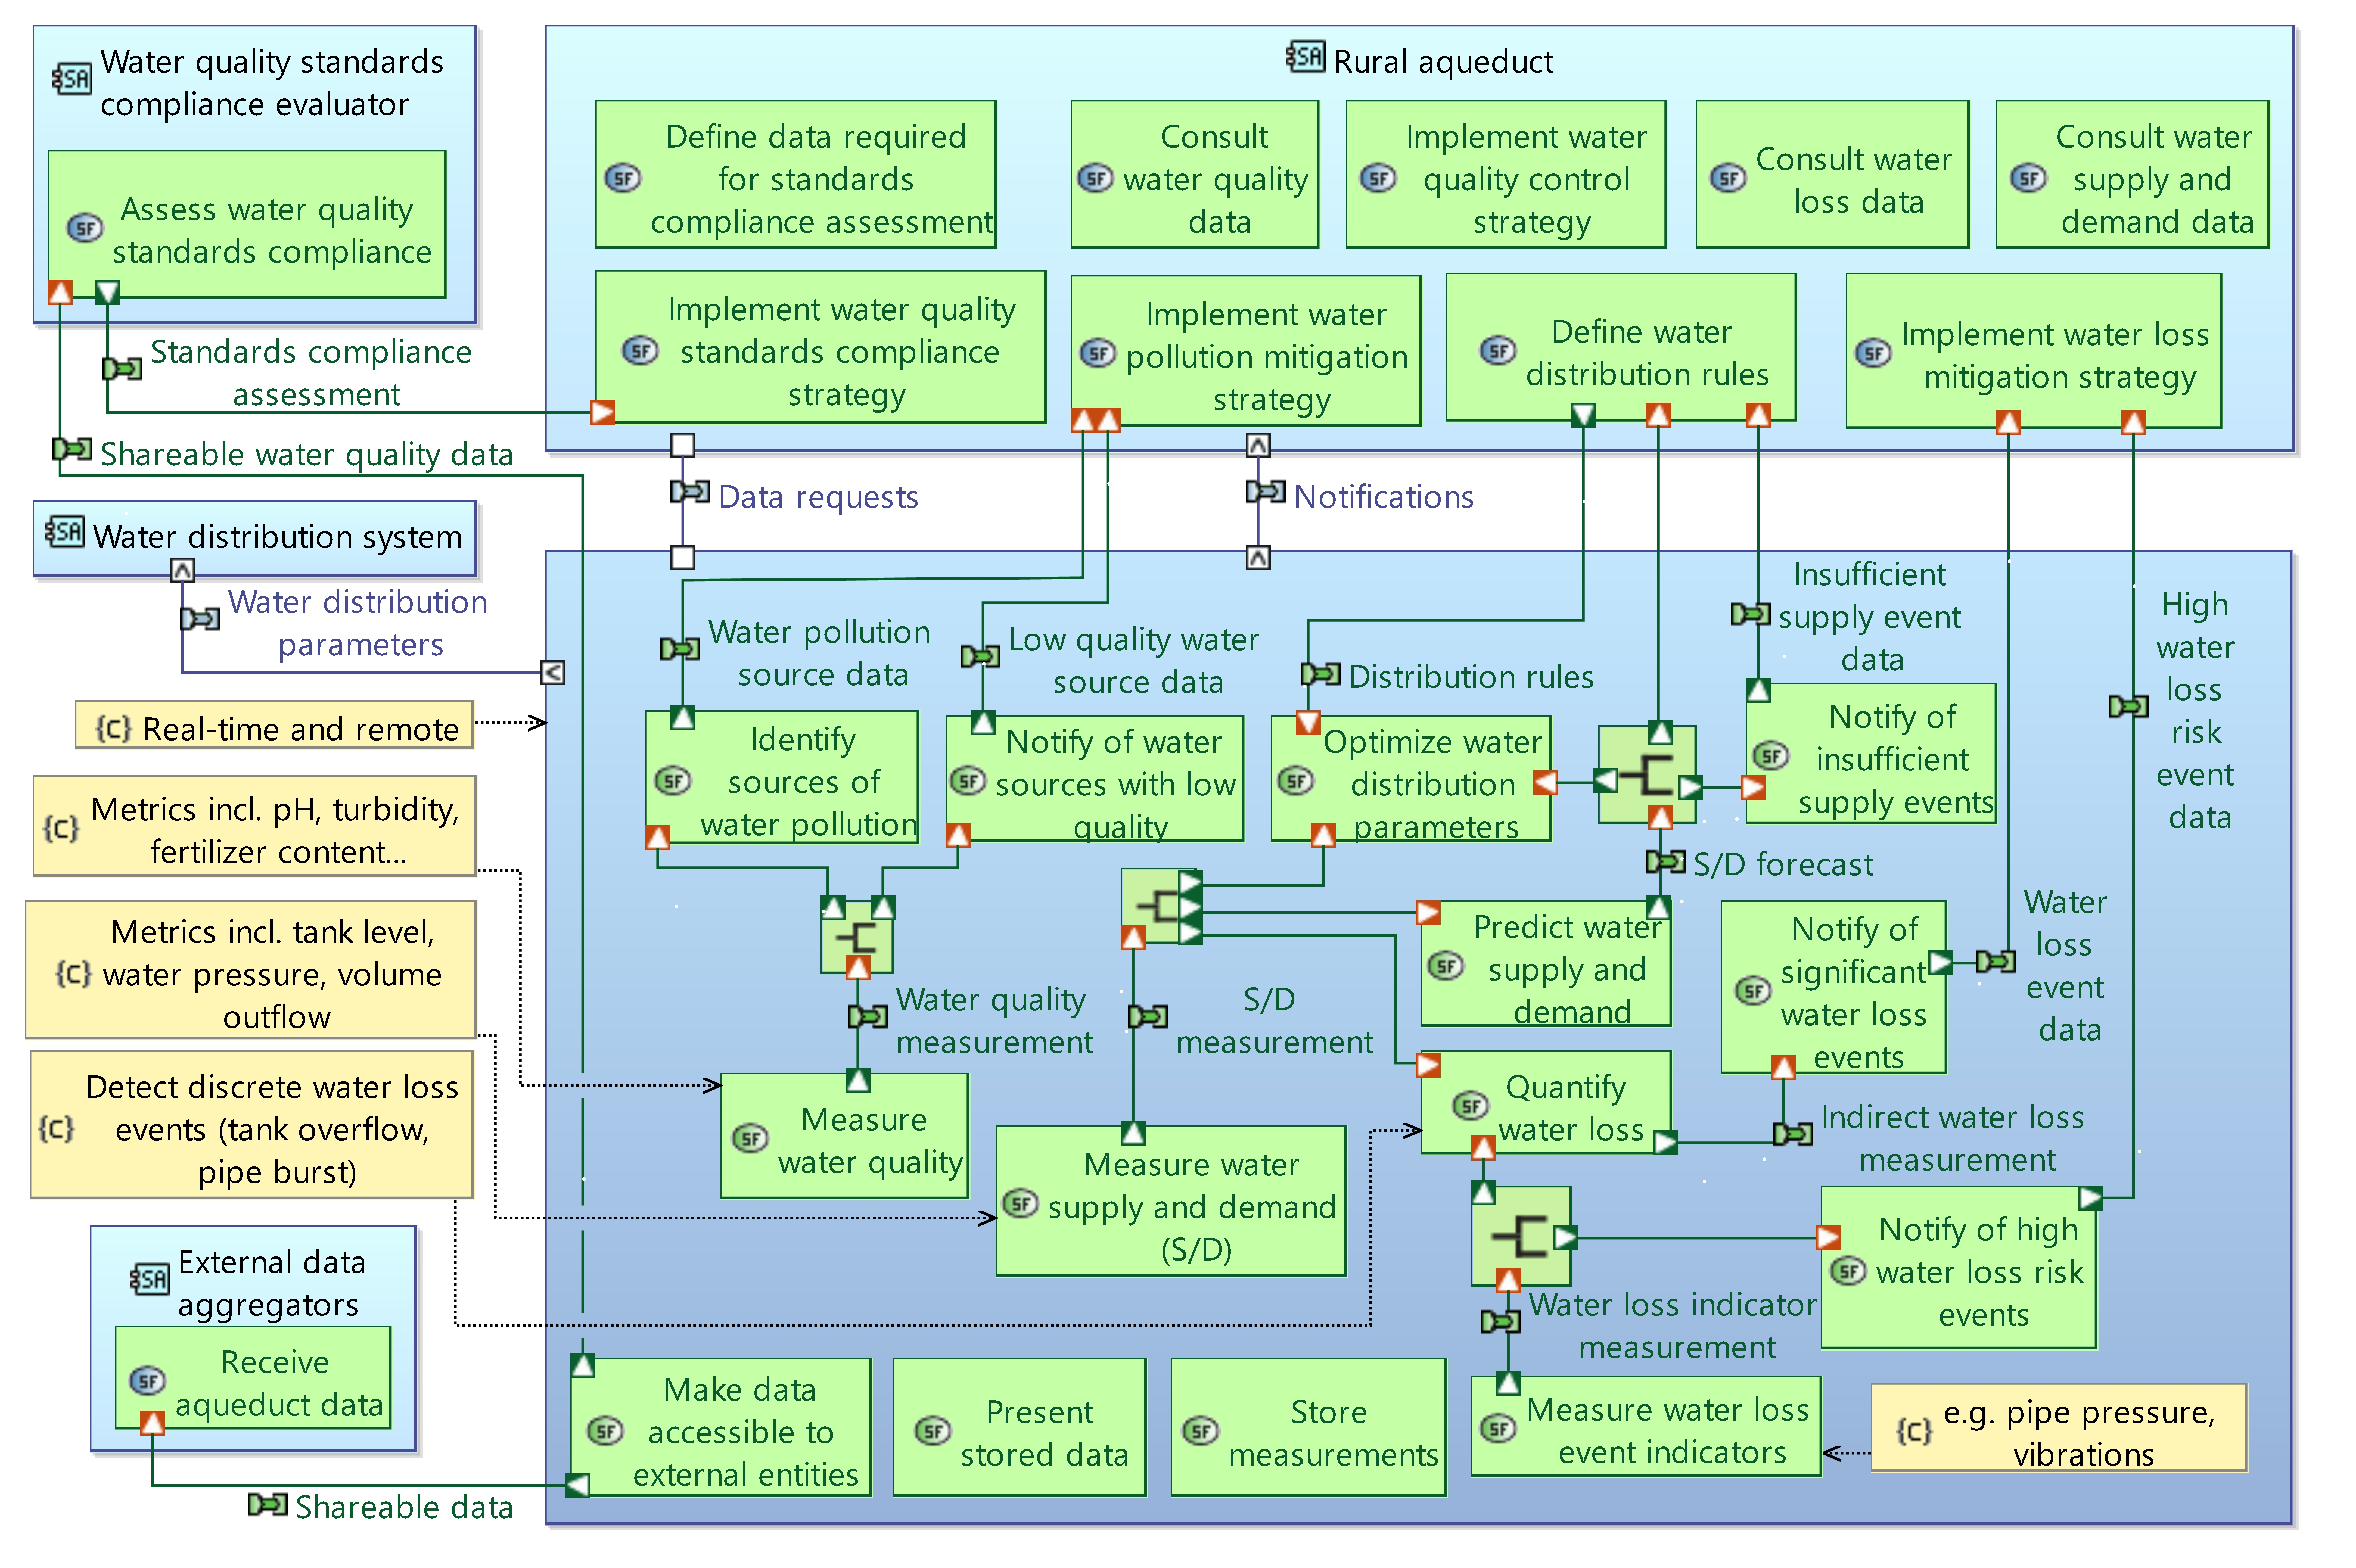
\includegraphics[width=\linewidth,scale= 0.9]{system_architecture.jpg}
    \caption{System needs analysis model of a generic and modular IoT system for rural aqueducts.}
    \label{fig:sab}
\end{figure*}

From this second perspective, monitoring activities are delegated to the system, while the organization’s role shifts to consulting the collected data and implementing strategies based on it. Modularity is incorporated by minimizing dependencies between functions across different system capabilities and by generalizing system functions to achieve high-level objectives through various methods and data sources. For example, the system function Measure water quality does not specify exact variables and metrics to maintain flexibility; however, common parameters identified in the literature—such as pH and turbidity—are included as constraints.

Another crucial implementation of modularity at the system needs analysis level is the separation of the water distribution system (WDS), hydraulic in nature, from the IoT system which is the focus of this work. To this purpose, the WDS is represented as an external entity for which only its interactions with the IoT system—water distribution parameters optimized by the latter—are constrained, while its internal functional content is recognized as out of scope.

Following the operational and system needs analysis, the design of the solution architecture proceeds with the definition of the logical architecture (Figure \ref{fig:la}). This logical structure describes the desired system behaviors necessary to meet user needs. At this stage, the system is decomposed into behavioral components, each with distinct functions. Through the interactions and functional exchanges among these components, the collective behavior required from the system is realized.

\begin{comment}
 In this second perspective, monitoring activities are now delegated to the system, while
the organization's role is simplified to consulting the collected data and implementing strategies
based on it. Modularity is imbued to the system by avoiding dependencies between
the functions belonging to different system capabilities as much as possible,
and by generalizing system functions so that they can fulfill a high-level objective via
different means and based on different sources of data.
For example, in the system function \textit{Measure water quality} the exact variables
and metrics that define water quality are left unspecified for greater flexibility,
yet common implementations identi+S/Dfied in the literature are presented as constraints (i.e. using pH and turbidity to determine quality).

After the operational and system needs analysis presented above, the solution
architecture design begins with defining the logical architecture (Figure \ref{fig:la}).
The logical structure of the system described the behaviors desired of it
so that it can fulfill the needs of its users.
At this point, the system is divided into behavioral componentes which are understood
to have different behaviors, yet through their individual functions and the
functional exchanges between them they give rise to the expected behavior of the
system as a whole.   
\end{comment}

\begin{figure*}[hbt]
    \centering
    
\includegraphics[width=0.98\linewidth,scale= 0.9]{logical_architecture.jpg}
    \caption{Logical architecture of a generic and modular IoT system for rural aqueducts. Some functional exchanges and logical actors are hidden for clarity.}
    \label{fig:la}
\end{figure*}

The modularity requirement influenced the logical architecture by separating the behavioral components that interact with end users from those that interface with the environment, while simplifying the former. This design allows data acquisition and processing components to be modified to include or exclude variables as needed, yet they consistently communicate with users through the more generic long-term storage, dashboard, and notifier components. These latter components maintain consistent behavior regardless of the number or type of variables monitored or the complexity of detected events, as they merely respond to user requests by presenting pre-existing data in predefined formats, such as notifications or dashboards.

Additionally, three important concepts supporting modularity are introduced through component exchanges: buses, queues, and publish/subscribe (pub/sub) channels, also called topics. Buses transport measurement data from sensors to the data acquisition subsystem via a multi-point interface, allowing sensors measuring different variables to be added or removed without affecting the underlying infrastructure.

Queues are first-in, first-out buffers that temporarily store data until the receiving component is ready to consume it. This decouples data processing components from the data-producing components, enabling measurements to be processed not individually, when
they lack context, but within a time window, by enabling the dedicated Measurement window
behavioral component to trigger event detection and processing tasks only when the measurement windows are fully populated.
Importantly, the rate at which windows populate is determined by user-configurable data collection frequencies and window sizes.

On a related note, pub/sub channels function as named queues that can be nested to represent hierarchies of variables, data streams, and events. Compared to queues, pub/sub channels generally involve higher latency and internet-based data transactions.

The generality and modularity of the proposed solution do not limit its value for potential IoT system designers, as it captures essential design guidelines within the component exchange models. Specifically, it requires that data transactions from acquisition and processing to long-term storage be enabled via a querying language. Moreover, the architecture prescribes routing all incoming user data requests through a dashboard, greatly simplifying user access control and interaction mechanisms.

\begin{comment}
The modularity viewpoint was taken into account with this logical architecture
by separating the behavioral components that interact with final users
from those that interact with the environment, and by simplifying the former.
This entails that the data acquisition and processing components can be modified
to include or exclude variables, yet they always interface with end users via
the more generic long-term storage, dashboard, and notifier components.
The latter three components do not change their behavior regardless of the nature
and amount of variables monitored by the system, or the complexity of the events
detected via data processing, because they must only respond to the requests from
the users of events generated within the system, by presenting pre-existing data
in a pre-defined format (a notification or a dashboard).

Furthermore, three important concepts for modularity are introduced in the form of component exchanges:
buses, queues, and pub/sub channels (also called topics).
Buses transport measurement information from sensors to the data acquisition subsystem, and they do so through
a multi-point interface from which sensors related different variables can be added or removed as per
the specific system requirements, without affecting the underlying infrastrcture.

Queues are first-in-first-out buffers of data points that can store data until the receiving component is ready
to process it.
This limits the functionality of data processing components to simply consuming data at the rate at which it is
available on the queue, without having to interact directly with the components that produce this data.
Lastly, pub/sub channels can be understood as queues with descriptive names, which can be nested to represent
hierarchies of variables, data streams, and events.
In pub/sub topics, data
creation and consumption usually have a much higher latency with respect to queues, and data transctions occur via the internet,

The generality and modularity of the solution are not to the detriment of its contribution
to potential IoT-system designers, as it encodes crucial design guidelines through the model element of component exchanges.
Namely, it specifies that regardless of the nature of the data being moved from the data acquisition and processing components
to long-term storage, the data transaction must be enabled by a querying language.
Furthermore, the architecture prescribes that all incoming user requests for data must be routed through a dashboard,
a choice that greatly reduces the complexity of defining how much access users should have into the system and the means
needed to enable it.   
\end{comment}



\subsection{An implementation on a real case study} 
To exemplify how the generic and modular IoT architecture presented in this work can be tailored to specific
contexts and configured for deployment, a physical IoT system architecture was developed for the rural aqueduct of ASADA
Paso Ancho, in the province of Cartago, Costa Rica.
The first step in this effort was to revise the operational analysis and preserve only the operational activities that this
aqueduct carries out, and similarly for the system needs.

This operational need-based refinement was carried out up to the physical architecture, which is presented in
Figure \ref{fig:pa}.
The main modification done to the logical architecture is the implementation of technology-specific needs and desires, exemplified in the
replacement of the sensor bus with the dedicated
electrical communication channels for the sensors already present at this rural aqueduct.
Also, physical components necessary for an actual on-site implementation where modeled and their functional and
non-functional requirements were stated, for example in the case of the solar powered battery that powers
the physical component (a microcontroller) that hosts the data acquisition and processing subsystems.

To show the modularity of the logical architecture, the long-term storage, dashboard, and notifier behavioral
components were moved to software server hosts, connected to the microcontroller deployed on-site via
mobile networks. This reduces physical and information technology maintenance costs for the rural aqueduct,
while also improving the system robustness by separating behaviors into physical components without a shared
failure mode.

\begin{figure*}[hbt] 
    \centering
    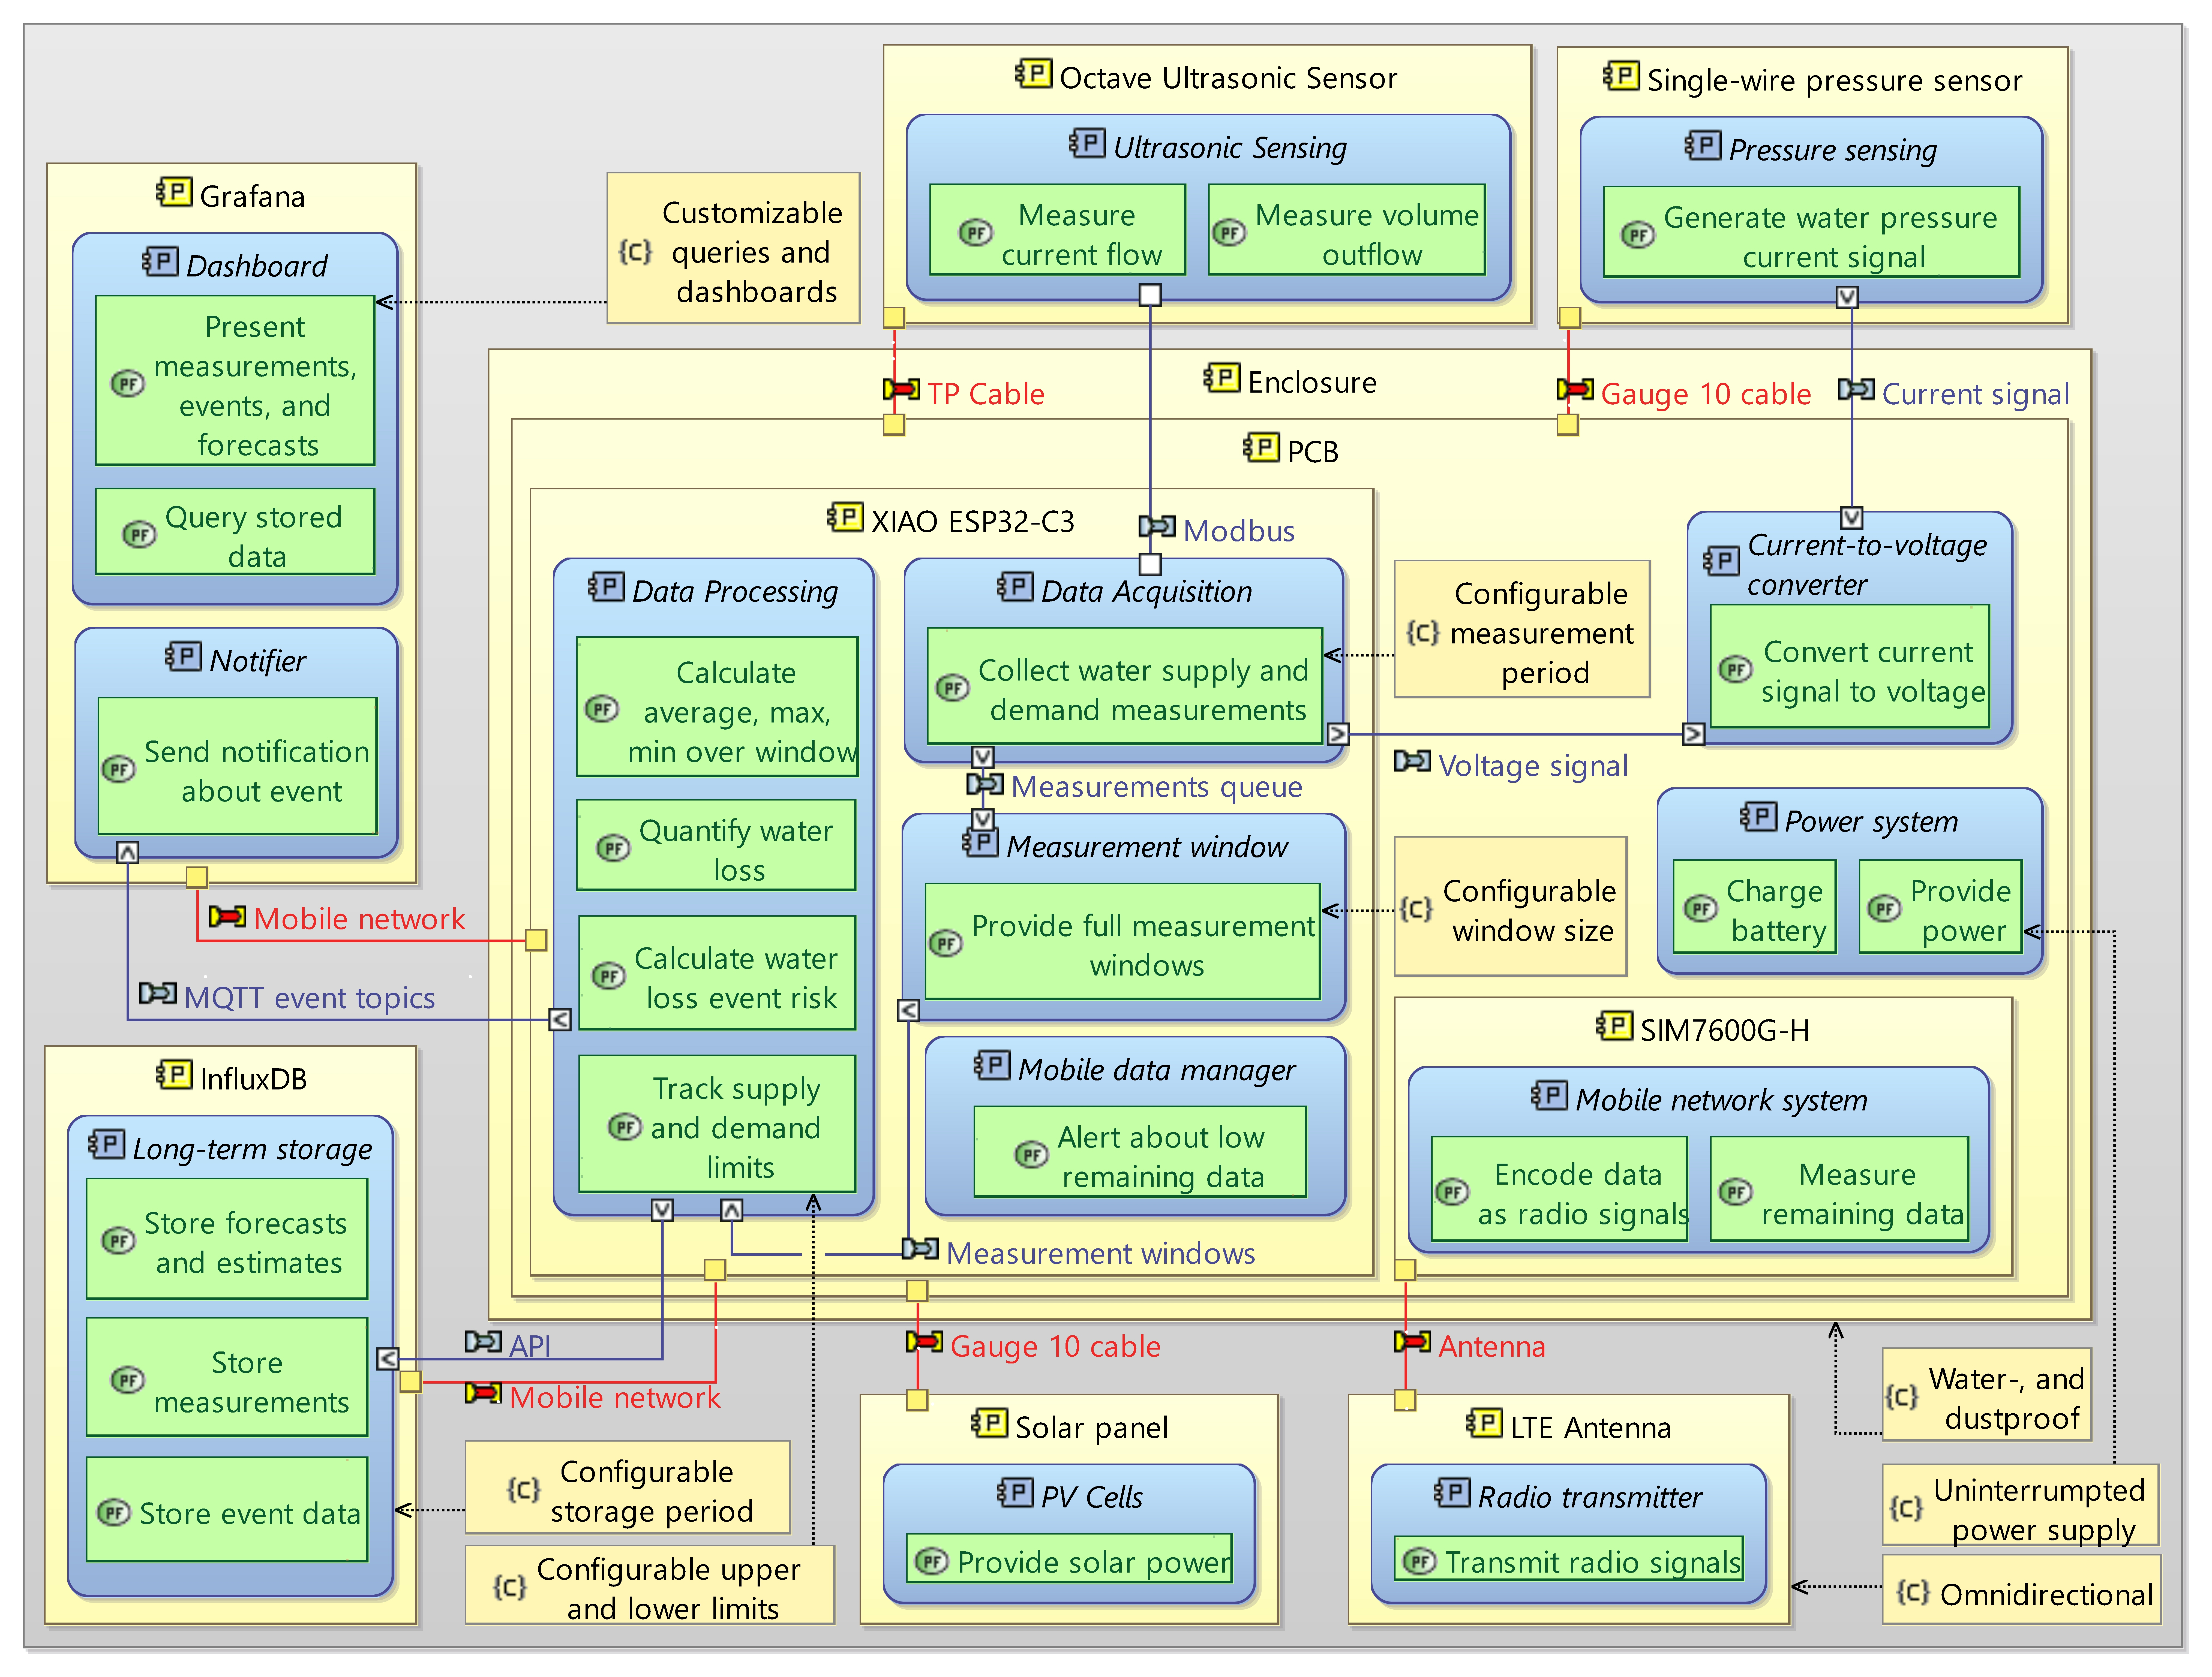
\includegraphics[width=0.9\linewidth] {physical_architecture.jpg}
    \caption{Physical architecture of an IoT system for ASADA Paso Ancho in Cartago, Costa Rica.}
    \label{fig:pa}
\end{figure*}

\section{Discussion}
The needs and desires extracted through data mining are representative of the general context of rural aqueducts. This is not only due to their alignment with findings from prior literature reviews \cite{w14223621} \cite{98953990}, but also because they were systematically derived from a substantial portion of the available academic work on the topic. Additionally, the use of BERTopic to represent thematic groupings helped weight these needs and desires by frequency, offering a proxy for their relative importance across rural aqueduct systems.

The systematic progression from needs and desires to solution architecture, as prescribed by the ARCADIA method, was essential in achieving robust generality. Rather than limiting requirement consideration to early design stages, the method ensures that these requirements are fulfilled by the final solution through explicit traceability from logical or physical architecture back to stakeholder needs. The concept of operational analysis also plays a critical role in demonstrating and communicating this generality, allowing readers to relate the engineering approach directly to their own context—free from the constraints of specific technology choices.

The generic operational need analysis revealed that rural aqueducts share a core set of activities, each governed by multiple non-functional requirements. For instance, the activity of monitoring water quality may involve variables ranging from turbidity and pH to bacterial presence. To support this diversity while preserving generality, non-functional requirements were assigned to the functions that can implement them. Enabling multiple configuration options in parallel required the component exchange between sensors and the data acquisition subsystem to be defined as a bus. This architecture allows data acquisition to interface with a wide range of sensors through shared physical connections, minimizing design complexity by ensuring uniform integration of compatible sensors.

The capability for pollution source identification further emphasizes the importance of modularity. This function depends on multiple sensor subsystems deployed across the aqueduct’s service area to add geospatial resolution to water quality data. The proposed architecture supports this by decoupling data acquisition and processing from long-term storage, enabling distributed sensing nodes while centralizing storage to handle high volumes of concurrent connections. Importantly, this configuration is only one of many viable implementations allowed by the logical architecture, which remains agnostic to specific technologies.

With regard to data flow, the use of measurement queues to decouple data
production and processing
is particularly relevant to the identified user desire of employing
machine learning and other processing-heavy methods for pollution source
and water loss event detection, among other tasks, in contrast to more lightweight and traditional rules-based approaches.
Furthermore, this separation is also crucial in allowing system designers to implement
the proposed architecture using wireless sensor networks, a common user need in the literature,
where measurement
nodes are commonly physically independent of data processing units yet operate
at a high frequency \cite{8308424}.

In the case of automatic water distribution control, the architecture introduces an important modularity consideration by modeling the physical distribution infrastructure (tanks, valves, pipes) as a separate entity from the core IoT system. This decision acknowledges that water distribution systems are an operational prerequisite for any rural aqueduct, even in the absence of digital systems. To maintain generality, the architecture avoids specifying detailed functional or non-functional characteristics of distribution systems. Instead, it focuses on ensuring integration by requiring that such systems be capable of receiving control commands via a pub/sub communication channel.

The role of functional and component exchanges within ARCADIA models must be emphasized. These exchanges define the interactions between system functions, while remaining open to further refinement at the logical architecture level.
This information not only informs the physical architecture but also clarifies external dependencies critical for system integration. As a result, individual functions or subsystems can be abstracted as self-contained modules—each potentially undergoing the ARCADIA method independently. This approach facilitates their development while positioning them as reusable, configurable components within broader IoT solutions, which, for example, would facilitate
adapting the Notifier, Event detection and Data processing components to generate new insights
based on the existing data flows, requiring substantially less adaptation effort compared
to an IoT system architecture not developed as an MBSE model.

\begin{comment}
The needs and desires extracted through data mining were representative of the general
context of rural aqueducts, not only because they match the findings of literature reviews
but because they were systematically derived from a significant percentage of the literature
on this topic. Furthermore, the BERTopic topic representations contributed to weighting
the individual needs and desires by frequency, and thus, by their importance for rural
aqueducts.

The systematic progression for needs and desires to solution architectures prescribed by ARCADIA was key in
obtaining robust generality, by avoiding a superficial consideration of requirements only at the early design stages
and instead ensuring that they are truly fulfilled by the finalized version of the solution,
by following the traceability links from the logical or even physical architecture upwards.
Also, the concept of operational analysis aids significantly in communicating and proving this generality, 
since readers can compare the requirements engineering presented here to their own context directly at the level
of needs and desires, with complex specifics like technology choices absent.

The generic operational need analysis showed that rural aqueducts implement a set of core activities,
but with multiple non-functional requirements for each.
For example, the generic activity of monitoring water quality is configurable to rely on variables from
turbidity and pH to bacterial proliferation.
To encompass all of these configuration options and preserve generality, non-functional requirements were assigned
to the functions they can be implemented in.
However, for multiple, or potentially all, of these configuration options to be implementable in parallel is that the component exchange between the sensors and data acquisition subsystems
was defined as a bus.
In this configuration, the data acquisition subsystem can collect measurements from multiple variables through shared physical communication sources, with a low design complexity since
all sensors that are compatible with the bus are interfaced in the same way.

Pollution source identification, specifically, is also closely dependent on modularity as it relies on multiple
sensor subsystems distributed over the service area of the rural aqueduct, so as to give a geospatial dimension
to the water quality data.
This requirement is satisfied in the proposed architecture by separating the data acquisition and processing from the long-term storage behavior, so that the former can be implemented across multiple nodes and the latter
on a more centralized data store with a high capacity for simultaneous connections.
Still, this is only one of the many approaches that the logical architecture allows, thanks to it being independent 
of technology choices.

With regards to automatic control of water distribution, the proposed architecture makes an important
modularity consideration by modeling the water distribution system (tanks, valves, pipes) as an entity separate
to the core IoT system as described by the operational need analysis.
This was motivated by the fact that for any rural aqueduct to be operational, a water distribution system is a
fundamental requirement, even if it's the only system deployed by the organization.
Thus, to avoid hindering the generality of the architecture by defining the functional and non-functional
characteristics of distribution systems, this work instead models the requirement for such systems to be integrated
into the IoT framework, namely, the capacity to receive control commands via a pub/sub channel.

As a final note on modularity, the importance of the information contained in the functional and component
exchanges of ARCADIA system models is to be pointed out.
These exchanges model the interactions between functions, which at the logical architecture level are left open
to further definition.
Thus, with this information in hand, the developers of the physical architecture and beyond are guided not only
towards what the system should do, but to the external dependencies it must take into account in order to be
effectively integrated into the system.
This enables a potential separation of each function or subsystem and its boundary as a new system that can undergo
the ARCADIA method by itself, not only to facilitate its development process but to frame it as a reusable,
configurable, or modular component.    
\end{comment}


\section{Conclusions and future work perspectives}
This work presented a generic and modular IoT system architecture for rural aqueducts, grounded in a systematic application of the ARCADIA Model-Based Systems Engineering method. By deriving needs and desires from a comprehensive literature-based data mining process, the solution addresses a broad spectrum of functional and non-functional requirements relevant to diverse rural contexts.

The ARCADIA method enabled a traceable and structured design process, ensuring that stakeholder needs are not only captured but also fulfilled throughout the logical and physical architecture stages. The operational analysis phase was particularly valuable in preserving generality, as it abstracted technological choices and allowed system designers to focus on what rural aqueducts must achieve, regardless of implementation constraints.

Modularity was a core design principle, reflected in the separation of user-facing and environment-interfacing components, the use of flexible communication models such as buses and pub/sub channels, and the definition of configurable system functions. This approach facilitates scalability, reusability, and adaptation to varying levels of technical capacity in rural settings.

Overall, the proposed approach provides a practical and adaptable foundation for developing IoT-based monitoring and control systems in rural aqueducts. It is further intended as a guideline for student-driven and academic technology transfer initiatives, fostering sustainable and context-aware digitalization in underserved water management systems.

Future work will focus on extending the identification and formalization of requirements through the use of text embeddings applied to a broader set of references. Additionally, further development of physical components with implementation-specific requirements is an opportunity to advance the proposed architecture into a complete, low-cost, and deployable solution for particular rural aqueducts.

\bibliographystyle{IEEEtran}
\bibliography{references, autorefs}

\end{document}
